\section{Extension to Distributed Memory}

\subsection{SDSM Framework Introduction}
\begin{frame}
    \frametitle{SDSM Framework}
    	Novel shared-distributed-shared-memory (SDSM) 
    	framework uses
    \begin{itemize}
    	\item Hierarchical dynamic load-balancing,
    	\item Work-stealing
    \end{itemize}
     	to balance the load among the processes for our CORDAC algorithms.
\end{frame}

\subsection{SDSM: Multi-level Hierarchy}
\begin{frame}
    \frametitle{Multi-level Hierarchy}
    If we have $K$ processes,
    \begin{itemize}
    	\item a super-master,
    	\item some $M'$ of them as masters, and
    	\item the rest as workers.
    \end{itemize}
    They run multithreaded code on $p$ cores.
\end{frame}

\begin{frame}
    \frametitle{Shared Job Queue}
    \begin{itemize}
    	\item Each super-master/master process maintains a shared 
    		job queue.
    	\item If a thread run a function on input size
            \footnote{$\textit{min offload threshold} \le x \le \textit{max offload threshold}$}
             $x$, 
    		try to lock the job queue and put at most $l-1$
    		out of its $l$ parallellly executable recursive sub-divisions in job queue.
    	\item If a thread waits its submitted jobs finished,
    		it steals back its latest submitted jobs left in the job queue.
    \end{itemize}
\end{frame}

\subsection{SDSM: Result}
\begin{frame}
    \frametitle{Result}
    \begin{figure}
		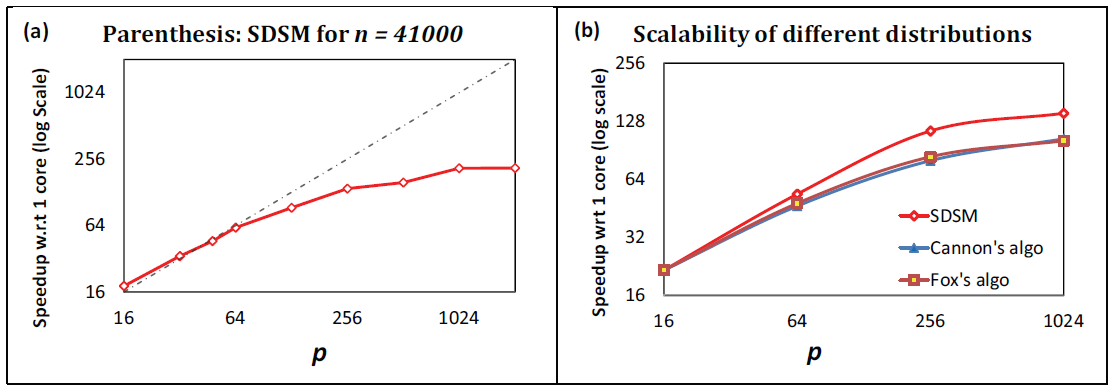
\includegraphics[scale=0.3]{figure/fig-distributed-result.png}
	\end{figure}
    \begin{itemize}
    	\item For parenthesization problem, we fixed $n = 41 K$ and 
    		allowed offloading of problems with a size in the range of
    		$256$ -- $2048$.
    \end{itemize}
\end{frame}